\documentclass[9pt,a4paper,landscape]{extarticle}

\usepackage{array}
\usepackage{url}
\usepackage{graphicx}
\usepackage[hmargin=0.5cm,vmargin=1.cm]{geometry}
\usepackage{stix}
\setlength{\extrarowheight}{.3pt}
\newcommand{\CC}{C\nolinebreak\hspace{-.05em}\raisebox{.3ex}{\footnotesize +}\nolinebreak\raisebox{.3ex}{\footnotesize +}}\renewcommand*{\UrlFont}{\ttfamily\small\relax}\begin{document}%
\thispagestyle{empty}%
\begin{minipage}{.5\textwidth}%
\begin{minipage}{.58\textwidth}{\Huge OpenDreamKit (ODK) Glossary}\end{minipage}\begin{minipage}{.3\textwidth}
\includegraphics[scale=0.14]{logos/odk.png}\hspace{.2\textwidth}
\includegraphics[scale=0.08]{logos/europe.png}\end{minipage}\vspace{.2cm}%

\begin{tabular}{@{}m{.13\textwidth}p{.77\textwidth}@{}}
\hline
{\large Anaconda} & 
\begin{tabular}{@{}p{.77\textwidth}@{}}
distribution of scientific softwares
\\ \url{https://www.continuum.io/}\end{tabular}
\\\hline
{\large API} & 
\begin{tabular}{@{}p{.77\textwidth}@{}}
Application Programming Interface: specifications of communication protocols between software components
\end{tabular}
\\\hline

\includegraphics[scale=0.35]{logos/binder.png} & 
\begin{tabular}{@{}p{.77\textwidth}@{}}
web-application for Jupyter notebook visualization from a github repository
\\ \url{http://mybinder.org/}\end{tabular}
\\\hline
{\large CAS} & 
\begin{tabular}{@{}p{.77\textwidth}@{}}
Computer Algebra System
\end{tabular}
\\\hline
{\large Conda} & 
\begin{tabular}{@{}p{.77\textwidth}@{}}
package management system used in Anaconda
\\ \url{https://conda.io/docs/}\end{tabular}
\\\hline
{\large Cygwin} & 
\begin{tabular}{@{}p{.77\textwidth}@{}}
collection of tools which provide Linux functionalities on Windows
\\ \url{https://www.cygwin.com}\end{tabular}
\\\hline

\includegraphics[scale=0.25]{logos/cythonlogo.png} & 
\begin{tabular}{@{}p{.77\textwidth}@{}}
optimising static compiler from Python to C
\\ \url{http://cython.org}\end{tabular}
\\\hline

\includegraphics[scale=.32]{logos/docker-logo.png} & 
\begin{tabular}{@{}p{.77\textwidth}@{}}
software container platform (alternative to VM)
\\ \url{https://www.docker.com}\end{tabular}
\\\hline
{\large findstat} & 
\begin{tabular}{@{}p{.77\textwidth}@{}}
collaborative database for combinatorial statistics
\\ \url{http://www.findstat.org/}\end{tabular}
\\\hline
{\large flint} & 
\begin{tabular}{@{}p{.77\textwidth}@{}}
C library for number theory
\\ \url{http://flintlib.org}\end{tabular}
\\\hline

\includegraphics[scale=0.12]{logos/gap.png} & 
\begin{tabular}{@{}p{.77\textwidth}@{}}
CAS for discrete computational algebra
\\ \url{https://www.gap-system.org}\end{tabular}
\\\hline

\includegraphics[scale=0.2]{logos/git-small.png} & 
\begin{tabular}{@{}p{.77\textwidth}@{}}
a version control system
\\ \url{https://git-scm.com/}\end{tabular}
\\\hline

\includegraphics[scale=0.32]{logos/github_logo.png} & 
\begin{tabular}{@{}p{.77\textwidth}@{}}
git based hosting service for software development
\\ \url{https://github.com}\end{tabular}
\\\hline
\begin{minipage}{.15\textwidth}
{\large gitlab}
\\
\includegraphics[scale=0.017]{logos/gitlab.png}
\end{minipage}&
\begin{tabular}{@{}p{.77\textwidth}@{}}
wiki and issue tracking system for software development projects (see also trac)
\\ \url{https://about.gitlab.com/}\end{tabular}
\\\hline
{\large HPC} & 
\begin{tabular}{@{}p{.77\textwidth}@{}}
High Performance Computing
\end{tabular}
\\\hline
\begin{minipage}{.15\textwidth}
{\large IPython}
\\
\includegraphics[scale=0.055]{logos/copie.png}
\end{minipage}&
\begin{tabular}{@{}p{.77\textwidth}@{}}
command shell for interactive computing
\\ \url{https://ipython.org}\end{tabular}
\\\hline
{\large JOOMMF} & 
\begin{tabular}{@{}p{.77\textwidth}@{}}
Jupyter-OOMMF
\\ \url{http://joommf.github.io}\end{tabular}
\\\hline

\includegraphics[scale=0.23]{logos/jupyter-small.png} & 
\begin{tabular}{@{}p{.77\textwidth}@{}}
web-application for interactive computations
\\ \url{http://jupyter.org/}\end{tabular}
\\\hline

\includegraphics[scale=0.12]{logos/jupyterhub.png} & 
\begin{tabular}{@{}p{.77\textwidth}@{}}
configurable multi-user Jupyter server
\\ \url{https://jupyterhub.readthedocs.io}\end{tabular}
\\\hline

\includegraphics[scale=0.32]{logos/linbox.png} & 
\begin{tabular}{@{}p{.77\textwidth}@{}}
exact linear algebra \CC{} library
\\ \url{http://www.linalg.org}\end{tabular}
\\\hline

\includegraphics[scale=0.23]{logos/lmfdb-logo.png} & 
\begin{tabular}{@{}p{.77\textwidth}@{}}
L-functions and Modular Forms Database: collaborative knowledge and data-base for number theory
\\ \url{http://www.lmfdb.org/}\end{tabular}
\\\hline
\begin{minipage}{.15\textwidth}
{\large MathHub}
\\
\includegraphics[scale=0.03]{logos/mathHubLogo.png}
\end{minipage}&
\begin{tabular}{@{}p{.77\textwidth}@{}}
portal for active mathematical documents and formalizations
\\ \url{https://mathhub.info}\end{tabular}
\\\hline
\end{tabular}%
\end{minipage}%
\begin{minipage}{.5\textwidth}%
\begin{tabular}{@{}m{.13\textwidth}p{.77\textwidth}@{}}
\hline
{\large MMT} & 
\begin{tabular}{@{}p{.77\textwidth}@{}}
Meta-Meta-Tool: data/knowledge/software management framework based on OMDoc/MMT
\end{tabular}
\\\hline
{\large MPIR} & 
\begin{tabular}{@{}p{.77\textwidth}@{}}
C library for multiprecision integer and rational arithmetic
\\ \url{http://mpir.org}\end{tabular}
\\\hline
{\large nbdime} & 
\begin{tabular}{@{}p{.77\textwidth}@{}}
notebook diffing and merging: Python library for version control for Jupyter notebooks
\\ \url{https://github.com/jupyter/nbdime}\end{tabular}
\\\hline
{\large nbval} & 
\begin{tabular}{@{}p{.77\textwidth}@{}}
Python library to test Jupyter notebooks
\\ \url{https://github.com/computationalmodelling/nbval}\end{tabular}
\\\hline

\includegraphics[scale=0.12]{logos/numpy.jpg} & 
\begin{tabular}{@{}p{.77\textwidth}@{}}
Python library for N-dimensional arrays and linear algebra
\\ \url{https://www.numpy.org}\end{tabular}
\\\hline
{\large OEIS} & 
\begin{tabular}{@{}p{.77\textwidth}@{}}
The On-Line Encyclopedia of Integer Sequences
\\ \url{https://oeis.org/}\end{tabular}
\\\hline
{\large OMDoc/MMT} & 
\begin{tabular}{@{}p{.77\textwidth}@{}}
Open Mathematical Documents / Meta Meta Theories: representation format
\\ \url{http://uniformal.github.io/doc/index.html}\end{tabular}
\\\hline
{\large OOMMF} & 
\begin{tabular}{@{}p{.77\textwidth}@{}}
Object Oriented MicroMagnetic Framework
\\ \url{http://math.nist.gov/oommf/}\end{tabular}
\\\hline
{\large OpenMath} & 
\begin{tabular}{@{}p{.77\textwidth}@{}}
extensible standard for representing the semantics of mathematical objects
\\ \url{http://openmath.org}\end{tabular}
\\\hline
{\large OpenMP} & 
\begin{tabular}{@{}p{.77\textwidth}@{}}
Open Multi-Processing: API for parallel programming
\\ \url{http://www.openmp.org}\end{tabular}
\\\hline

\includegraphics[scale=0.22]{logos/logo_pari_gp.png} & 
\begin{tabular}{@{}p{.77\textwidth}@{}}
C library for number theory and command line interface
\\ \url{https://pari.math.u-bordeaux.fr}\end{tabular}
\\\hline

\includegraphics[scale=0.085]{logos/python.png} & 
\begin{tabular}{@{}p{.77\textwidth}@{}}
programming language and interpreter
\\ \url{https://www.python.org}\end{tabular}
\\\hline
\begin{minipage}{.15\textwidth}
{\large Pythran}
\\
\includegraphics[scale=0.35]{logos/pythran-logo-small.png}
\end{minipage}&
\begin{tabular}{@{}p{.77\textwidth}@{}}
Python to \CC{} compiler for a subset of the Python language
\\ \url{https://pythonhosted.org/pythran}\end{tabular}
\\\hline

\includegraphics[scale=0.1]{logos/sage_logo.png} & 
\begin{tabular}{@{}p{.77\textwidth}@{}}
CAS which aggregates dozens of other softwares and libraries such as FLINT, GAP, LinBox, MPIR, PARI/GP, Singular
\\ \url{http://www.sagemath.org}\end{tabular}
\\\hline

\includegraphics[scale=0.17]{logos/sphinx.png} & 
\begin{tabular}{@{}p{.77\textwidth}@{}}
software to create documentation
\\ \url{http://www.sphinx-doc.org/en/stable/}\end{tabular}
\\\hline
\begin{minipage}{.15\textwidth}
{\large SMC}
\\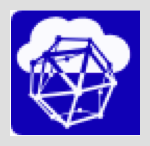
\includegraphics[scale=0.25]{logos/SMC-bis.png}
\end{minipage}&
\begin{tabular}{@{}p{.77\textwidth}@{}}
SageMathCloud: web-appliction and website for collaborative work around SageMath, Jupyter, LaTeX, \ldots
\\ \url{https://cloud.sagemath.com}\end{tabular}
\\\hline

\includegraphics[scale=0.22]{logos/scipy.png} & 
\begin{tabular}{@{}p{.77\textwidth}@{}}
Python libraries for mathematics, science, and engineering
\\ \url{https://scipy.org}\end{tabular}
\\\hline
{\large SCSCP} & 
\begin{tabular}{@{}p{.77\textwidth}@{}}
Symbolic Computation Software Composability Protocol
\end{tabular}
\\\hline
{\large SIMD} & 
\begin{tabular}{@{}p{.77\textwidth}@{}}
Single Instruction Multiple Data (in-core parallelism)
\end{tabular}
\\\hline

\includegraphics[scale=4]{logos/singular.jpg} & 
\begin{tabular}{@{}p{.77\textwidth}@{}}
CAS for commutative algebra and algebraic geometry
\\ \url{https://www.singular.uni-kl.de}\end{tabular}
\\\hline
{\large SGE} & 
\begin{tabular}{@{}p{.77\textwidth}@{}}
Son of Grid Engine and derivatives: distributed resource manager and batch job scheduler for HPC clusters
\\ \url{https://arc.liv.ac.uk/trac/SGE}\end{tabular}
\\\hline

\includegraphics[scale=0.25]{logos/trac.png} & 
\begin{tabular}{@{}p{.77\textwidth}@{}}
wiki and issue tracking system for software development projects (see also gitlab)
\\ \url{https://trac.edgewall.org/}\end{tabular}
\\\hline
{\large VM} & 
\begin{tabular}{@{}p{.77\textwidth}@{}}
Virtual Machine: software that emulates a computer in an operating system
\end{tabular}
\\\hline
{\large VRE} & 
\begin{tabular}{@{}p{.77\textwidth}@{}}
Virtual Research Environment
\end{tabular}
\\\hline
\end{tabular}%
\end{minipage}%
\end{document}
